\documentclass[twoside]{book}
\usepackage[top=0.9in, bottom=0.9in,left=0.9in, right=0.9in, paperwidth=6in, paperheight=9in]{geometry}
\usepackage{puzzles}

\begin{document}
\title{Математические головоломки}
\author{Питер Винклер}
\date{}
\maketitle

\chapter*{Интуиция}
 

\epigraph{Когда напряженная умственная работа сменяется периодами отдыха, интуиция словно берет верх, и порождает кристально ясные откровения, привносящие в процесс научного исследования неповторимое удовольствие и наслаждение.}{Фритьоф Капра, физик}

Эта глава предназначена для разминки и содержит задачи, не относящиеся к какой-либо специфической теме или технике.
Однако, как часто бывает в таких случаях, некоторые ключевые идеи могут помочь вам в дальнейшем.
 Вот для начала одна из подобных задач:

\subsection*{Монеты в ряд} %(COINS IN A ROW)

На столе выложен ряд из пятидесяти монет различного достоинства.
Алиса берет монету с одного конца и кладет себе в карман, затем Боб выбирает монету с одного из концов, и так они продолжают по очереди, пока Боб не забирает последнюю монету.

Докажите, что Алиса может вести игру таким образом, что, по крайней мере, сможет набрать денег не меньше, чем Боб.

\medskip

Попробуйте сыграть в эту игру сами, для начала с несколькими монетами (или случайными числами), начните с 4 или 6 вместо 50.
Совсем неочевидно, как играть оптимально, не так ли?
Но, может Алисе и не нужна оптимальная стратегия? 

Сейчас у Вас подходящий момент установить себе правило --- пытаться решить задачу до того, как вы продолжите чтение.

\paragraph{Решение:}
Пронумеруем все монеты от 1 до 50 и заметим, что, независимо от того, как ходит Боб, Алиса может забрать все чётные или, если она предпочитает, все нечётные монеты.
Один из этих выборов должен, по крайней мере, не уступать другому.
\heart

Эту задачу я узнал от Эхуда Фридгута;
говорят, что её давали при приеме на работу в одной израильской ИТ компании.
Вообщем-то у Алисы есть более оптимальные стратегии, чем выбор всех чётных или нечётных монет.
Заметим, однако, что если у нас 51 монета вместо 50, то Боб (игрок, который ходит вторым) обычно обладает преимуществом, несмотря на меньшее, чем у Алисы, количество собранных монет.
Кажется парадоксальным, что чётность числа монет имеет такой огромный эффект на результат игры, при том, что монеты берутся только с концов.

\medskip

Ну что ж, попробуйте теперь сами.
Мы начнем с двух менее математических задач, а затем перейдем к вещам посерьезнее.
И~пусть ваше воображение укажет вам верный путь!

\subsection*{Два Биксби} %(THE BIXBY BOYS)

Это был первый день школы и Миссис Фелдман, войдя в класс, увидела сидящих за первой партой двух абсолютно одинаковых учеников, Дональда и Рональда Биксби.

--- Вы двойняшки, не так ли? --- спросила она.

--- Нет, --- ответили они хором.

Миссис Фелдман проверила записи в журнале и убедилась, что у мальчиков одни и те же родители и родились они в один и тот же день.
Как такое может быть?

\subsection*{Свет на чердаке} %(THE ATTIC LAMP SWITCH)

На первом этаже дома находится панель с тремя выключателями, один из них включает свет на чердаке --- но который? 
Ваша задача --- совершить некие действия с выключателями и после одного похода на чердак определить, какой выключатель подключен к чердачной лампочке.

\subsection*{Бензиновый кризис} %(GASOLINE CRISIS)

Представьте, что у нас кризис --- не хватает бензина.
Заправочные станции, расположенные на большой кольцевой дороге, обладают все вместе количеством бензина, достаточным только для одного проезда по кольцу.
Докажите, что, отправившись с правильной автозаправки с пустым баком, вы сможете проехать по всей кольцевой дороге.

\subsection*{Бикфордовы шнуры} %(USES OF FUSES)

У вас имеются два бикфордовых шнура (т.~е. два куска огнепроводного шнура), каждый из них сгорает ровно за одну минуту, но горение неравномерно по длине шнура.
Можно ли при помощи этих двух бикфордовых шнуров отмерить 45 секунд?

\subsection*{Целые числа и прямоугольники} %(INTEGERS AND RECTANGLES)

Большой прямоугольник на плоскости разбит на малые прямоугольники, у каждого из которых либо высота, либо основание, либо оба --- целое число. 
Докажите, что большой прямоугольник также обладает этим свойством.

\begin{figure}[h!]
\centering
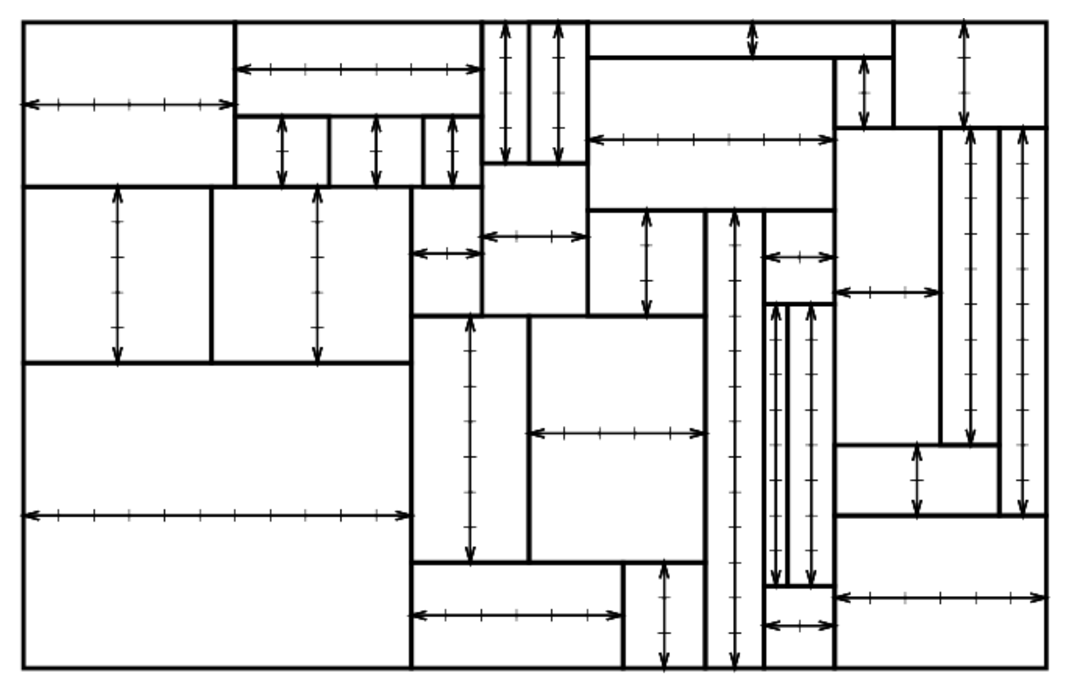
\includegraphics[scale=0.6]{Figs/Insight/rect}
\end{figure}

\subsection*{Весы и гири} %(TIPPING THE SCALES)

На столе у учителя стоят чашечные весы, правая чашка весов перевешивает.
На весах стоят гири не обязательно одного веса, на каждой из которых написаны фамилии одного \emph{или нескольких} учеников.
Ученик, входя в класс, переставляет на другую чашку весов каждую гирю, на которой написана его фамилия.
Докажите, что можно впустить в класс таких учеников, чтобы в результате перевесила левая чашка весов.

\subsection*{Часы на столе} %(WATCHERS ON THE TABLE)

На столе лежат пятьдесят точных ручных часов.
Докажите, что существует момент времени, когда сумма расстояний от центра стола до кончиков минутных стрелок больше, чем сумма расстояний от центра стола до центров часов.

\subsection*{Путь по шахматной доске} %(PATH ON CHESSBOARD)

Алиса начинает игру и ставит фишку в угол шахматной доски размером $n{\times}n$ клеток.
Боб передвигает фишку на соседнее поле, имеющее общую сторону с тем, на котором стоит фишка.
Второй раз ходить на поле, где уже побывала фишка, нельзя. 
Алиса и Боб ходят по очереди.
Проигрывает тот, кому некуда ходить.

При каких $n$ у Алисы есть выигрышная стратегия? 
При каких $n$ она выигрывает, если ее первый ход не на угловое поле, а на соседнее с ним?

\subsection*{Степень в степени} %(EXPONENT UPON EXPONENT)

На экзамене по математике для старших классов Американской школы 1960-х годов 
был следующий вопрос:
Если 
$$x^{x^{x^{{\cdot}^{\cdot^{\cdot}}}}}=2$$
Чему равен $x$? 
Предполагаемое решение основывается на том, что степень «нижнего» $x$ равна всему выражению, таким образом $x^2\z=2$ и $x=\sqrt{2}$.
Но один ученик заметил, что если бы в задаче спрашивалось решение
$$x^{x^{x^{{\cdot}^{\cdot^{\cdot}}}}}=4$$
то он бы получил тот же ответ: $x=\sqrt[4]{4}=\sqrt{2}$

Хмм...
Чему же тогда равно ${\sqrt{2}}^{{\sqrt{2}}^{{\sqrt{2}}^{{\cdot}^{\cdot^{\cdot}}}}}$? 
Можете это доказать?

\subsection*{Солдаты в поле} %(SOLDIERS IN THE FIELD)

Нечётное число солдат расположилось на поле таким образом, что все попарные расстояния между ними (между каждой парой солдат) различны.
При этом каждый солдат должен присматривать за ближайшим к нему другим солдатом.

Докажите, что существует хотя бы один солдат, за которым никто не присматривает.

\subsection*{Отрезки и расстояния} %(INTERVALS AND DISTANCES)

Пусть множество $S$ состоит из $k$ непересекающихся отрезков, лежащих в единичном отрезке $[0,1]$.
Предположим, что $S$ обладает следующим свойством: для любого вещественного числа $d$ из отрезка $[0,1]$, в множестве $S$ существуют две точки на расстоянии $d$ друг от друга.
Докажите, что сумма длин отрезков $S$ не меньше $1/k$.

 
\subsection*{Собрать 15} %(SUMMING TO 15)

Алиса и Боб по очереди выбирают число из $1, 2,\dots,9$, без повторов.
Выигрывает тот, кто первый наберет три числа, дающие в сумме 15.
Имеется ли у Алисы (она ходит первая)
выигрышная стратегия?

%ё
\section*{Решения и комментарии}

\subsubsection*{Два Биксби} % (THE BIXBY BOYS)

Классическая головоломка.
Конечно же, это были тройняшки.
Третий близнец (Арнольд?) учился в другом классе.

\subsubsection*{Свет на чердаке} % (THE ATTIC LAMP SWITCH)

Эта задача пронеслась по миру, как эпидемия гриппа, где-то лет десять тому назад; я не знаю её источника.

Действительно, невозможно определить, какой выключатель подключён к лампочке на чердаке, если всё, что у вас имеется --- это один бит информации, полученный от вашего похода на чердак.
Однако, вы можете добыть больше сведений, если используете ваши руки!
Включите выключатели 1 и 2, подождите несколько минут, затем выключите второй выключатель и идите на чердак.
Если лампочка не горит, но горячая, значит, второй выключатель это то, что мы ищем.
\heart

Если вы не можете дотянуться до лампочки, но обладаете огромным терпением, вы можете добиться того же результата, включив второй выключатель и подождав пару месяцев, затем включить первый выключатель и посетить чердак.
Если лампочка перегорела, то виноват в этом второй выключатель.

\subsubsection*{Бензиновый кризис} %(GASOLINE CRISIS)

Эта задача была известна довольно давно, вы можете найти её, например, в чудесной книге Ласло Ловаса\footnote{Laszlo Lovasz, \emph{Combinatorial Problems and Exercises}.}.
Трюк заключается в следующем:
представьте, что вы начинаете на автозаправке, скажем, №\,1 с достаточным количеством бензина и затем продолжаете свой путь, опустошая каждую автозаправку на кольцевой дороге.
Когда вы вернётесь к заправке №\,1, 
у вас будет столько же бензина, как и в начале пути.

Во время поездки записывайте, сколько бензина у вас остаётся перед каждой заправочной станцией.
Предположим, что это количество минимально перед автозаправкой №\,$k$.
Значит, если вы начнёте с автозаправки №\,$k$ с пустым баком, вы не рискуете оказаться без бензина на дороге между заправочными станциями.\heart

\subsubsection*{Бикфордовы шнуры} %(USES OF FUSES)

Подожгите одновременно оба конца первого шнура и один конец второго.
Когда первый шнур сгорит (через полминуты), подожгите незажжённый конец второго шнура.
К моменту, когда он догорит полностью, пройдёт 45 секунд.
\heart

Несколько лет назад эта и другие задачи о бикфордовых шнурах распространились по миру, как лесной пожар.
Дик Хесс, эксперт по занимательной математике, 
собрал небольшую книжку таких задач.\footnote{Dick Hess and Jerry Slocum, \emph{Shoelace Clock Puzzles}.}
Сам он впервые услышал приведённую выше задачу от Карла Морриса из Гарвардского университета.

Хесс рассматривает бикфордовые шнуры (он их зовёт шнурками) различной длины, но поджигает их только с концов.
Если же вам позволено поджигать шнур во внутренних точках и вы обладаете определённой ловкостью, то можно добиться гораздо большего.
Например, можно отмерить 10 секунд с помощью одного 60-секундного шнура, если зажечь его с обеих концов и в двух внутренних точках, а затем, каждый раз, когда сегмент сгорает, поджигать в новой внутренней точке.
Таким образом, у вас всё время горят три сегмента с двух концов, и шнур сгорает в шесть раз быстрее.

Будет немного суеты под конец и, конечно же, понадобится бесконечное число спичек, чтобы достичь абсолютной точности.

\subsubsection*{Целые числа и прямоугольники} %(INTEGERS AND RECTANGLES)}

Эта задача была предметом особой 
статьи Стэна Вэгона.%
\footnote{Stan Wagon “Fourteen proofs of a Result about Tiling a Rectangle”, American Mathematical Monthly Vol. 94, (1987) pp 601--617.}

Некоторые из решений, предложенных Вэгоном, забавным образом используют мощную математическую технику.
А одно решение не из их числа, предлагает нам следущее:
наложим на большой прямоугольник сетку, состоящую из квадратов со стороной 1/2, так, чтобы нижний левый угол прямоугольника находился в вершине клетки сетки.
Раскрасив клетки сетки в белый и чёрный цвета в шахматном порядке, 
мы видим, что каждый малый прямоугольник ровно наполовину белый и наполовину чёрный.
Следовательно, то же будет верно и для большого прямоугольника.
Но, допустим, высота большого прямоугольника не целое число, тогда часть 
большого прямоугольника между линиями $x=0$ и $x=1/2$ не содержит одинаковое количество белого и чёрного цвета.
Следовательно, основание должно быть целым числом.\heart

Автор книги несёт ответственность за следующее решение, которое вы не найдёте в статье Вэгона.
Пусть $\varepsilon$ меньше, чем наименьшая допустимая длина стороны прямоугольника разбиения.
Раскрасим каждый малый прямоугольник с целым основанием зелёным цветом, кроме красных горизонтальных полосок шириной $\varepsilon$ вдоль его верхней и нижней сторон.
Раскрасим оставшиеся прямоугольники красным, за исключением зелёных вертикальных полосок шириной $\varepsilon$ вдоль левой и правой сторон.

%в решении ссылаются на цвета диаграмы, но при печати она станет ч/б
\begin{figure}[h!]
\centering
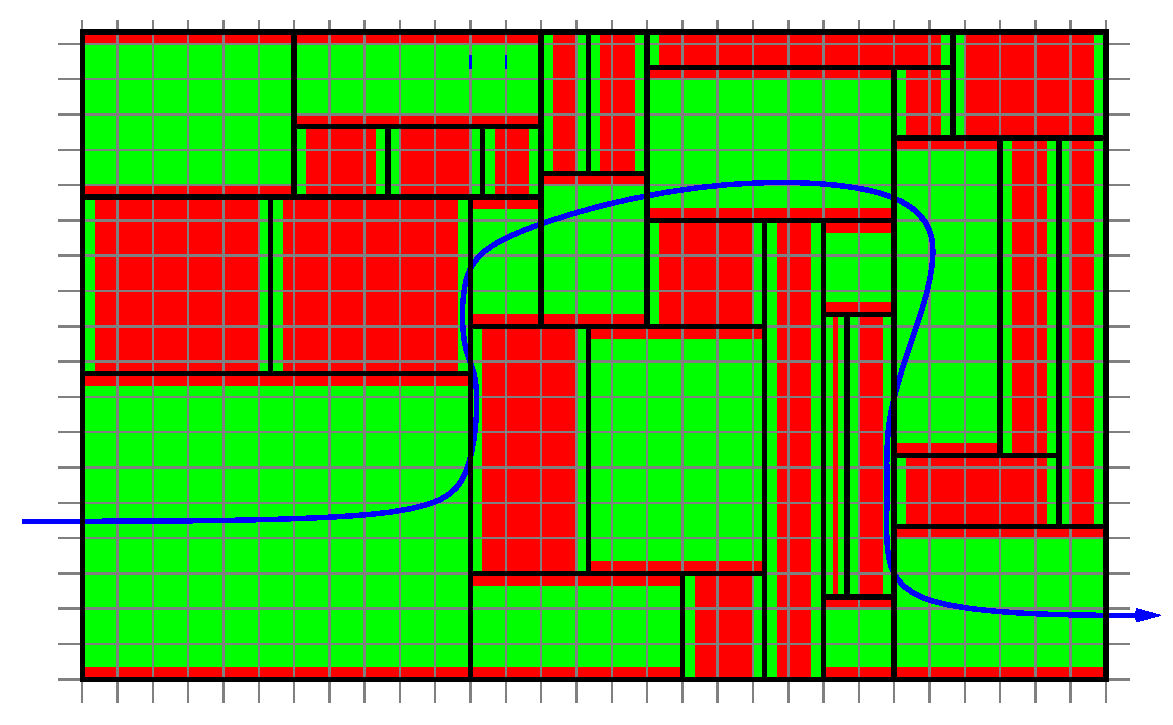
\includegraphics[scale=0.5]{Figs/Insight/green}
\end{figure}

Поместим в нижний левый угол большого прямоугольника начало координат.
Заметим, что у нас есть либо зелёный путь с левой стороны большого прямоугольника до его правой стороны, либо красный путь с нижней стороны до верхней.
Рассмотрим первый вариант.
Каждое место пересечения зелёного пути с вертикальными сторонами малых прямоугольников имеет целую координату; таким образом, основание большого прямоугольника --- целое число.
Подобным же образом и красный путь снизу вверх определяет целую высоту.

\subsubsection*{Весы и гири} %(TIPPING THE SCALES)

Рассмотрим результат для каждого подмножества учеников, включая пустое.
Заметьте, что каждая гиря окажется на левой чашке весов ровно в половине случаев.
В частности, средний вес гирь на левой чашке для всех подмножеств учеников равен их среднему весу на правой чашке.
Поскольку для пустого множества правая чашка тяжелее, 
для какого-то другого множества тяжелее должна быть левая.\heart

\noindent{\small Источник: Вторая Всесоюзная математическая олимпиада, Ленинград, 1968.}

Техника «усреднения», описанная выше, часто используется: будьте внимательны!

\subsubsection*{Часы на столе} %(WATCHERS ON THE TABLE)

Рассматривая только одни часы, 
мы видим, что в течении одного часа среднее расстояние от центра стола $C$ до кончика минутной стрелки $M$ превышает расстояние от $C$ до центра часов $W$.
Действительно, если провести через точку $C$ прямую $L$, перпендикулярную прямой $CW$, 
то среднее расстояние от прямой $L$ до точки $M$, очевидно, равно $LW$, 
что, в свою очередь, равно $CW$.
Но расстояние $CM$, по меньшей мере, равно $LM$, а обычно больше.

Взяв сумму по всем часам, приходим к аналогичному заключению, и отсюда следует, что есть момент в течении одного часа, когда желанное неравенство выполняется.\heart

\begin{figure}[h!]
\centering
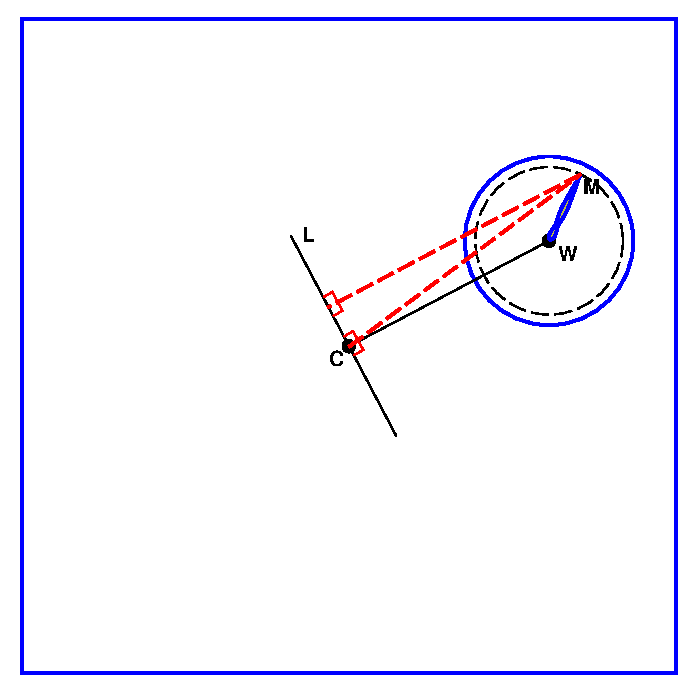
\includegraphics[scale=0.9]{Figs/Insight/watch}
\end{figure}

Требование точности часов обеспечивает движение каждой минутной стрелки с постоянной скоростью.
Это не так уж важно, когда скорости различаются, если только наше терпение не ограничено одним часом.

Одно дополнительное замечание: если установить и расположить часы определённым образом,
то \emph{можно} добиться того, что сумма расстояний от центра стола до кончиков минутных стрелок всегда была строго больше, чем сумма расстояний от центра стола до центров часов.\heart

\noindent{\smallИсточник: данная задача впервые появилась на десятой Всесоюзной математической олимпиаде в Душанбе, 1976.}

\subsubsection*{Путь по шахматной доске} %(PATH ON CHESSBOARD)

Если $n$ --- чётное число, у Боба имеется простая выигрышная стратегия, независимо от того, где Алиса начинает.
Он просто представляет себе, что шахматная доска покрыта прямоугольничками размером $1{\times2}$ клетки (домино) и каждый раз ставит фишку на вторую клетку того домино, куда пошла Алиса («закрывает» домино). %???обычно говорят «доминошки»
(Заметим, что эта стратегия работает для Боба, даже если Алисе разрешено ставить фишку на любую клетку при каждом ходе!).

Если $n$ --- нечётное, и Алиса начинает с угла, она выигрывает, если представит, что домино покрывает всю доску, кроме угловой клетки, с которой она начинает.

Tем не менее, Алиса проигрывает в случае с нечётным $n$, если она должна начинать с клетки, соседней к угловой.
Предположим, угловые клетки на данной доске чёрные, то есть Алиса начинает с белой клетки.
Существует покрытие всей шахматной доски домино, за исключением одной чёрной клетки.
Боб выигрывает, «закрывая» все домино.
Алиса
никогда не сможет поставить фишку на незакрытую клетку, потому что все клетки, на которые она ходит --- белые.\heart

\noindent{\small Источник: Двенадцатая Всесоюзная математическая олимпиада, Ташкент, 1978.}

\subsubsection*{Степень в степени} %(EXPONENT UPON EXPONENT)

Если выражение
$${\sqrt{2}}^{{\sqrt{2}}^{{\sqrt{2}}^{{\cdot}^{\cdot^{\cdot}}}}}$$
имеет какой-то смысл, то это не что иное, как предел последовательности
$${\sqrt{2}}, {\sqrt{2}}^{{\sqrt{2}}}, {\sqrt{2}}^{{\sqrt{2}}^{{\sqrt{2}}}},\dots$$
Этот предел существует, так как последовательность возрастает и ограничена.

Для доказательства первого утверждения, обозначим эту последовательность
$s_1, s_2,\dots$ и докажем по индукции, что $1<s_i\z<s_{i+1}$
для каждого $i\ge 1$.
Это сделать легко, поскольку \[s_{i+2}=
{\sqrt{2}}^{s_{i+1}}
>{\sqrt{2}}^{s_{i}}
=s_{i+1}.\]

Для нахождения верхней грани, заменим самую верхнюю степень в каждом $s_i$ на б\'{о}льшее число $2$, тогда всё выражение превращается в двойку.

Теперь, когда мы знаем, что предел существует, обозначим его $y$.
Он должен удовлетворять уравнению ${\sqrt{2}}^y=y$.
Рассмотрев уравнение $x=y^{1/y}$, 
можно увидеть, применив элементарный матанализ (приношу извинения!), 
что $x$ строго возрастает при возрастании $y$ до максимума при $y=e$
и после чего убывает.
Таким образом, существует не больше двух значений $y$, для данного $x$, 
и при $x=\sqrt{2}$ нам известны оба: $y=2$ и $y=4$.

Поскольку наша последовательность ограничена сверху двойкой, можно исключить $4$ и, таким образом, $y=2$.\heart

Обобщив приведённое выше доказательство, мы видим, что выражение $x^{x^{x^{{\cdot}^{\cdot}}}}$
имеет смысл и равно наименьшему решению уравнения $x=y^{1/y}$ при $x\le e^{1/e}$.
При $x=e^{1/e}$, выражение равно $e$ но как только $x$ превысит $e^{1/e}$, последовательность устремляется к бесконечности.

\subsubsection*{Солдаты в поле}%(SOLDIERS IN THE FIELD)

Данная задача была представлена на шестой Всероссийской математической олимпиаде в Воронеже, 1966.
Её легче всего решать, начав с двух солдат, находящихся друг от друга на кратчайшем расстоянии.
Ясно, что они присматривают друг другом, и если кто-то ещё смотрит на одного из них, тогда у нас имеется солдат, за которым присматривают дважды и, значит, есть солдат, за которым никто не присматривает.
Если же за этими двумя солдатами больше никто не присматривает, то можно их убрать, не влияя на остальных.

Так как число солдат нечётное, то, применяя и далее это рассуждение, мы, в конце концов, придём к одному солдату, который ни за кем не присматривает --- противоречие.\heart

\subsubsection*{Отрезки и расстояния} %(INTERVALS AND DISTANCES)

{\small Источник: Семнадцатая Всесоюзная математическая олимпиада, Кишинёв, 1983.}

Обозначим через $s_1,\dots,s_k$ длины отрезков множества $S$,
пусть их сумма равна $s$.
Рассмотрим интервал $I_{ij}$, содержащий все расстояния, которые можно получить, взяв первую точку на $i$-том и вторую на $j$-том отрезке множества $S$.
Ясно, что длина $I_{ij}$ равна $s_i+s_j$.
Суммируя по всем парам $i\ne j$, 
каждая длина появляется $k-1$ раз,
таким образом, сумма длин интервалов по всем парам различных отрезков, не превосходит $(k-1) s$.
Расстояния между точками, взятыми из $i$-ого отрезка, имеют значения от $0$ до $s_i$.
Значит, общая длина всех интервалов $I_{ij}$ не превосходит $k s$.
Поскольку $k s\ge 1$, получаем $s\ge 1/k$.
\heart

Равенство достигается, если максимум всех $s_i$ равен $s$, 
то есть если все отрезки, кроме одного, имеют нулевую длину.
Этого можно добиться взяв отрезок $[0,\tfrac1k]$ и добавив изолированные точки
$\tfrac2k,\tfrac3k,\dots,1$.

%исправлена фактическая ошибка --- отрезок можно брать только с краю, в середине брать нельзя.

\subsubsection*{Собрать 15} %(SUMMING TO 15)

Быстрый способ решить данную задачу --- это представить, что Алиса и Боб пользуются следующим магическим квадратом:
$$
\begin{matrix}
8&1&6\\
3&5&7\\
4&9&2
\end{matrix}
$$
Так как числа в строчке, столбике и диагонали дают в сумме 15, то можно сказать, что они играют в крестики-нолики! 
Всем известно, что наилучшая игра в крестики-нолики приводит к ничьей,
то есть ответ на наш вопрос --- нет, у Алисы нет выигрышной стратегии.
\heart

Эта забавная игра упоминается во втором томе классической книги Элвина Берлекампа, Джона Конвея и Ричарда Гая.\footnote{Winning Ways for Your Mathematical Plays by Elwyn Berlekamp, John Conway and Richard Guy ; Academic Press, 1982: 2nd Edition, A K Peters 2001}
В книге задача приписывается некоему «Э. Периколозо Спорджерси»\footnote{E. Pericoloso Sporgersi}, что выглядит очень подозрительно --- такую надпись можно увидеть в итальянских поездах, она предупреждает пассажиров об опасности высовываться из окна.

\end{document}
%ссылки на источник даются в разном формате, я бы его униформуизировал 
%проверь разбивку на абзацы, иногда она у тебя не та, что у винклера 